\subsection{Ingresos y egresos}

\subsubsection{Ingresos}

El plan de negocio propone dos fuentes principales de ingresos. La primera proviene de la publicidad, dirigida a aquellos interesados en adquirir implementos que optimicen su rendimiento físico. Para ello, se ofrece un plan de suscripción publicitaria para gimnasios, tiendas de ropa y equipos deportivos, suplementos y productos de nutrición, dispositivos de seguimiento de fitness, alimentos saludables, así como eventos y competencias deportivas.

La segunda fuente de ingresos proviene de los planes de acceso al producto. El plan gratuito se ofrece en formato de prueba, destinado a personas que desean explorar el servicio antes de comprometerse. Por otro lado, el plan mensual formaliza el interés del cliente en el negocio, permitiéndole acceder a los beneficios completos del servicio. En la tabla \ref{ingresos} se presenta un desglose más detallado, que incluye el análisis mensual y anual por compañía.

\vspace{2mm}
\begin{minipage}{0.9\textwidth}
\centering
\captionof{table}[{Ingresos}]{ Ingresos. }
\label{ingresos}
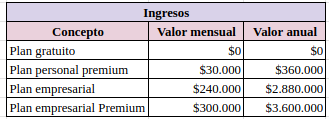
\includegraphics[width=0.7\textwidth]{Images/ingresos.png}
\fnote{Nota. \textup{Fuente : Autores}}
\end{minipage}


\subsubsection{Egresos}
En el primer año, se considera a las dos personas que lideran el proyecto, operando con un equipo reducido, quienes recibirán sus pagos conforme a las prestaciones sociales y aportes parafiscales estipulados por la normativa colombiana. Además, se contempla la infraestructura de trabajo virtual como parte de los gastos operativos. En la tabla \ref{egresos} se detalla más a fondo esta información.

\vspace{2mm}
\begin{minipage}{0.9\textwidth}
\centering
\captionof{table}[{Egresos}]{ Egresos. }
\label{egresos}
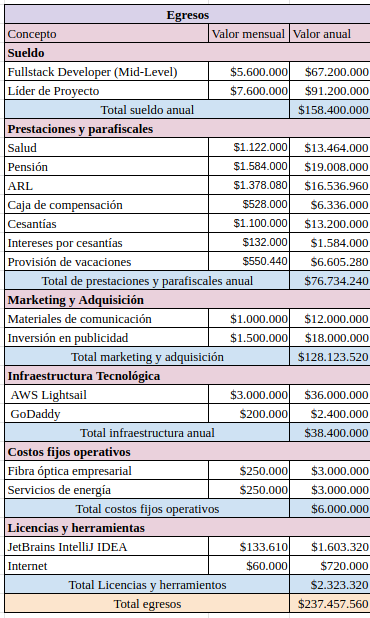
\includegraphics[width=0.7\textwidth]{Images/egresos.png}
\fnote{Nota. \textup{Fuente : Autores}}
\end{minipage}